% !TEX encoding = UTF-8
% !TEX TS-program = pdflatex
% !TEX root = ../../tesi.tex

\section{Integrazione del prodotto in NFTLab}
Dopo aver concluso. validato e collaudato la libreria, ho proceduto con l'integrazione di quanto fatto nel resto della piattaforma NFTLab. Come detto nella sezione precedente, è stato utilizzato lo \textit{smart contract} sviluppato in Solidity per Ethereum. \\

La piattaforma NFTLab si compone di due \textit{front-end} implementati utilizzando, rispettivamente, Angular e Vue.js. Il \textit{back-end} invece, dovrà comunicare con i \textit{front-end} sviluppati e gestire i dati delle opere che verranno salvate anche in \textit{blockchain} attraverso la libreria che ho prodotto. Questa inizia ad interagire sin dal primo accesso alla piattaforma NFTLab, infatti le immagini che vengono mostrate nella \textit{home} (figura \ref{nftlab:home}) vengono prelevate attraverso il servizio Pinata dalla rete IPFS.

% \clearpage
\begin{figure}[h!]
  \centering
  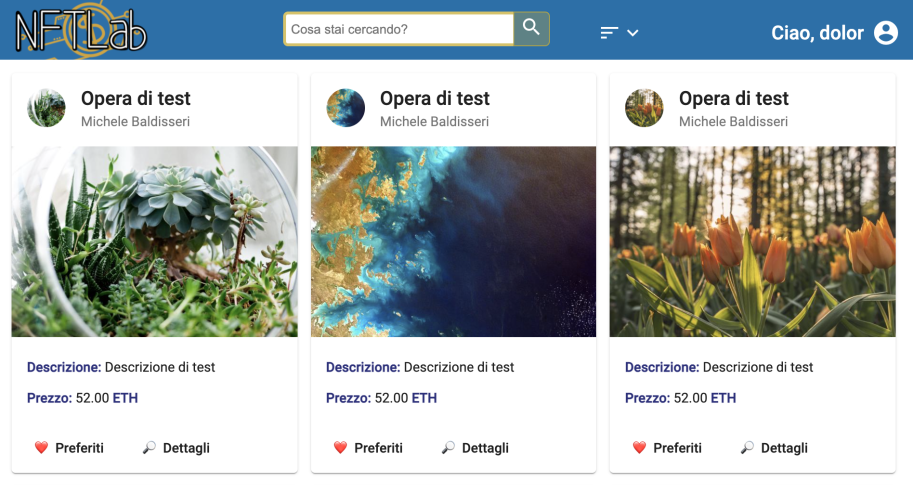
\includegraphics[width=0.9\textwidth]{capitolo3/prodotto-finale/home2.png}
  \caption{\textit{Home} della piattaforma NFTLab}
  \label{nftlab:home}
\end{figure}

Per quanto riguarda il caricamento di una nuova opera da parte di un utente autenticato, con relativa creazione del NFT, tutte le informazioni aggiuntive che vengono inserite nell'opportuna pagina (figura \ref{nftlab:upload-new-nft}), vengono salvate nel \textit{database} del \textit{back-end}. Allo \textit{smart contract} caricato in \textit{blockchain}, invece, si inviano solamente i dati più importanti, come la data di creazione e il \textit{wallet} dell'autore, per far si che abbiano valenza legale. Inoltre l'opera viene anche caricata nella rete IPFS e creato il NFT dal codice hash ricevuto.

\begin{figure}[h!]
  \centering
  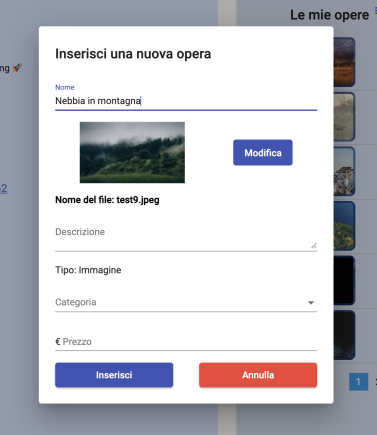
\includegraphics[width=0.5\textwidth]{capitolo3/prodotto-finale/upload-nft.png}
  \caption{Creazione di una nuova opera della piattaforma NFTLab}
  \label{nftlab:upload-new-nft}
\end{figure}

Il trasferimento della proprietà di un NFT non è ancora stato integrato dato che la rispettiva funzionalità al \textit{front-end} e \textit{back-end} non è stata implementata. Attualmente quest'ultima ha il compito di salvare i dati dell'acquirente, del venditore, la data di trasferimento e il prezzo, sempre per una questione di valenza legale.
